\subsubsection{User Story}
\textit{Diamond Stay} là một hệ thống trung gian giữa người cần thuê nhà và người cho thuê nhà. Hệ thống sẽ thu phí hoa hồng mỗi khi có lượt giao dịch thành công giữa chủ nhà và người cho thuê. Chủ nhà muốn thêm chỗ ở mới cần cho thuê thì cần gửi yêu cầu thêm chỗ ở mới lên hệ thống. Để thông tin về chỗ ở mới này xuất hiện trên trang web chính của \textit{Diamond Stay} để khách thuê nhà có thể thấy và đặt phòng thì tin đăng này cần phải được duyệt trước để đảm bảo tin đăng là hợp lệ, không phải là spam hay tin giả do một số đối tượng cố tình phá hoại hệ thống gửi lên. Những tin đăng loại này sẽ gây loãng hệ thống và gây khó khăn cho người dùng. Việc duyệt tin sẽ được những quản lí của hệ thống thực hiện. Hệ thống sẽ có một số tiêu chí để xác định tin đăng là hợp lệ hay không. Dựa vào đó quản lí có thể dựa vào để có thể quyết định trạng thái kế tiếp của 1 tin đăng. Các trạng thái này có thể là:
\begin{itemize}
	\item \textit{Thành công}: Tin đăng hợp lệ và được hiển thị lên trang web của Diamond Stay để khách thuê có thể nhìn thấy và đặt phòng 
	\item \textit{Bị từ chối}: Tin đăng không hợp lệ.
	\item \textit{Yêu cầu chỉnh sửa}: Tin đăng cần sửa đổi, bổ sung một số thông tin để hợp lệ. Chủ nhà sau khi sửa đổi và bổ sung có thể resubmit lại tin này.
\end{itemize}
Khi quản lí duyệt một tin là \textit{Bị từ chối} thì quản lí cần cung cấp lí do tin đăng bị từ chối, còn nếu tin đăng bị đánh giá là \textit{Yêu cầu chỉnh sửa} thì quản lí cần cung cấp chi tiết những nội dung nào cần chỉnh sửa, những nội dung nào chưa hợp lệ.
\subsubsection{Các usecase chi tiết}
\begin{figure}[!h]
	\centering
	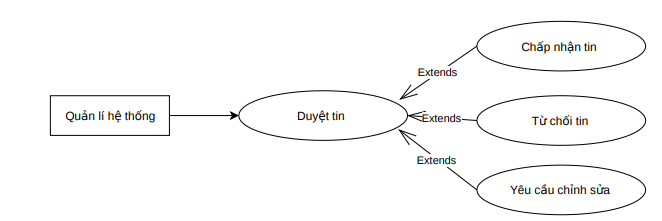
\includegraphics[width=12cm]{Image/module1.png}
	\vspace{0.5cm}
	\caption{Lược đồ use case của Module 1: Duyệt tin đăng yêu cầu thêm chỗ ở mới từ chủ nhà}
\end{figure}
\subsubsubsection{Use Case 1: Duyệt tin.}
\begin{figure}[!h]
	\centering
	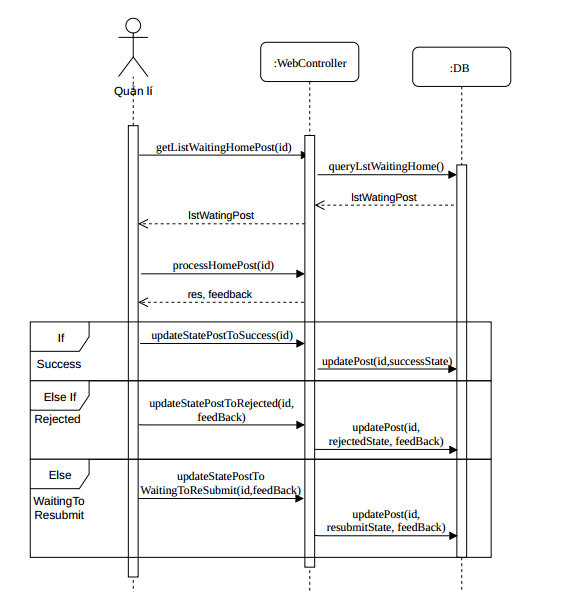
\includegraphics[width=13cm]{Image/duyetTinSequence.png}
	\caption{Sequence Diagram cho usecase Duyệt tin}
\end{figure}
\begin{center}
	\begin{longtable}{ | l |p{10cm}|}
		\hline
		\textbf{Tên usecase} & Duyệt tin \\ \hline
		\textbf{Người tương tác} & Quản lí hệ thống \\ \hline   
		\textbf{Mô tả} &  Cho phép người quản lí của hệ thống có thể duyệt qua các yêu cầu thêm nhà mới từ các chủ nhà. Việc duyệt tin để đảm bảo chất lượng của các bài đăng trên trang web của hệ thống.\\ \hline  
		\textbf{Người tạo:} \textit{Đinh Minh Tân} & \textbf{Cập nhật lần cuối bởi:} \textit{Đinh Minh Tân} \\ \hline
		\textbf{Ngày tạo:} \textit{22/03/2019} & \textbf{Lần cuối cập nhật:} \textit{30/03/2019} \\ \hline
		\textbf{Tiền điều kiện} &  Người dùng đã đăng nhập vào hệ thống bằng quyền của người quản lí, người dùng đang ở màn hình index của trang web. \\ \hline 
		\textbf{Hậu điều kiện} &  Quản lí quay về màn hình quản lí các tin chưa duyệt. \\ \hline 
		\textbf{Luồng cơ bản} & 
		\begin{enumerate}
			\item Quản lí nhấn tab Quản lí tin đăng.
			\item Hệ thống hiển thị 2 option cho quản lí bao gồm: Tin chưa duyệt, Tin đã duyệt.
			\item Quản lí chọn Tin chưa duyệt.
			\item Hệ thống hiển thị danh sách các tin chưa được duyệt, đang đợi duyệt.
			\item Người quản lí chọn một tin bất kì mà mình sẽ duyệt trong danh sách tin hiện ra.
			\item Hệ thống hiển thị tất cả thông tin của homestay cần được duyệt, trong đó có 3 option để duyệt: Chấp nhận, Từ chối và Yêu cầu chỉnh sửa.
			\item Quản lí sau khi duyệt tất cả các thông tin đầy đủ và hợp lệ, chọn option Chấp nhận và nhấn Button OK để xác nhận quyết định.
			\item Hệ thống hiện ra thông báo đã xác nhận thành công và tin đăng về homestay đã được đăng thành công lên trang web để khách thuê có thể thấy và đặt.
			\item Hệ thống quay về màn hình quản lí các tin chưa duyệt để quản lí có thể duyệt tin khác (nếu cần).
		\end{enumerate} \\ \hline 
		\textbf{Luồng thay thế} & 
		\begin{itemize} 
			\item \textit{Luồng thay thế 1}
			\begin{enumerate}
				\item Tại bước 4, hệ thống không tìm được tin nào chưa được duyệt thì sẽ in ra thông báo "Không có tin đăng nào cần duyệt" kết thúc chức năng này tại đây.
			\end{enumerate}
			
			\item \textit{Luồng thay thế 2}
			\begin{enumerate}
				\item Tại bước 6, quản lí chọn option Từ chối.
				\item Hệ thống hiện thị một form để quản lí điền lí do tin đăng bị từ chối. Sau khi hoàn thành xong form, quản lí nhấn OK.
				\item Hệ thống xác nhận tin đã bị từ chối và gửi kết quả về cho chủ nhà 
				\item Tiếp tục tại bước 9 của luồng cơ bản.
			\end{enumerate}
			
			\item \textit{Luồng thay thế 3}
			\begin{enumerate}
				\item Tại bước 6, quản lí chọn option Yêu cầu sửa đổi.
				\item Hệ thống hiện thị một form để quản lí điền những yêu cầu mà chủ nhà cần sửa đổi hoặc bổ sung thêm. Sau khi hoàn thành xong form, quản lí nhấn OK.
				\item Hệ thống đánh dấu chuyển tin sang dạng đợi và chuyển vào mục tin cần sửa đổi và resubmit lại bên phía chủ nhà.
				\item Tiếp tục tại bước 9 của luồng cơ bản.
			\end{enumerate}
		\end{itemize} \\ \hline 
		\textbf{Ngoại lệ}  & Không có \\
		\hline
	\end{longtable}
\end{center}